\documentclass[10pt]{article}
%----------------------------------------------------------------------------------------
%	Packages
%----------------------------------------------------------------------------------------
\usepackage[version=3]{mhchem} % Package for chemical equation typesetting
\usepackage{siunitx,enumitem} % Provides the \SI{}{} and \si{} command for typesetting SI units
\usepackage{graphicx} % Required for the inclusion of images
\usepackage{natbib} % Required to change bibliography style to APA
\usepackage{nth}
\usepackage{amsmath} % Required for some math elements
\usepackage{tabulary} % table package
\usepackage{graphicx}
\usepackage{floatrow} % change the placement of table caption heading
\usepackage{float} % controls the placement of figures
\usepackage[backend=biber,style=alphabetic]{biblatex}
\usepackage{chemfig} % use Chemistry symbols
\usepackage[font={small}]{caption}
\usepackage[margin=1in]{geometry}
\usepackage{array} % helps with wrapping text in columns
\usepackage{gensymb} % has the degree symbols
%----------------------------------------------------------------------------------------
%	Other Resources
%----------------------------------------------------------------------------------------
\addbibresource{cit.bib}
\setlength\parindent{0pt} % Removes all indentation from paragraphs
\newcolumntype{C}[1]{>{\arraybackslash}p{#1}}
\providecommand{\e}[1]{\ensuremath{\times 10^{#1}}}
% \renewcommand{\labelenumi}{\alph{enumi}.} % Make numbering in the enumerate environment by letter rather than number (e.g. section 6)

%\usepackage{times} % Uncomment to use the Times New Roman font

%----------------------------------------------------------------------------------------
%	Title, Name, Date, Partner, Instructor
%----------------------------------------------------------------------------------------
\title{Calcium in Soil\\ CHEM 1211L} % Title

\author{Chris \textsc{West}} % Author name

\date{\today} % Date for the report

\begin{document}

\maketitle % Insert the title, author and date

\begin{center}
\begin{tabular}{l r}
Date Performed: & June 26, 2017 \& June 28, 2017 \\% Date the experiment was performed
Partner: & Chris Tillis \\ % Partner names
Instructor: & Dr. MacGowan % Instructor/supervisor
\end{tabular}
\end{center}
\floatsetup[table]{capposition=top}
%\ce{Cu^2+}
%----------------------------------------------------------------------------------------
%	Abstract
%----------------------------------------------------------------------------------------
% \begin{abstract}

% \end{abstract}
%----------------------------------------------------------------------------------------
%	SECTION 1
%----------------------------------------------------------------------------------------

\section{Experimental Data and Calculations}
\begin{table}[H]
\label{Table 1}
\caption{Soil Preparation Data}
\resizebox{35em}{!}{
\begin{tabular}{|l|l|l|}
\hline
\multicolumn{1}{|c|}{{\ul{\textbf{Soil #}}}} &
\multicolumn{1}{c|}{{\ul{\textbf{Mass of Soil (grams)}}}} &
\multicolumn{1}{c|}{{\ul{\textbf{Amount of distilled \ce{H_2O}}}}}\\ \hline
	 1 & 5.06 & 100.5\\ \hline
	 3 & 5.05 & 100.0 \\ \hline
	\end{tabular}
	}
	\centering
\end{table}

\begin{table}[H]
\label{Table 2}
\caption{Experimental Parameters for \ce{Ca} titration of the soil's filtrate with EDTA}
\resizebox{40em}{!}{
\begin{tabular}{|l|l|l|l|l|l|}
\hline
\multicolumn{1}{|c|}{{\ul{\textbf{Molarity of EDTA (M)}}}} &
\multicolumn{1}{C{5.5cm}|}{{\ul{\textbf{Indicators Name $\&$ Amount used per titration(drops)}}}} &
\multicolumn{1}{C{5.5cm}|}{{\ul{\textbf{Buffer solution's pH $\&$ Amount used per titration (mL)}}}} &
\multicolumn{1}{C{5.5cm}|}{{\ul{\textbf{Vol. of distilled \ce{H_2O} used per titration(mL)}}}} &
\multicolumn{1}{c|}{{\ul{\textbf{mL of soil eluent}}}} &
\multicolumn{1}{C{5.5cm}|}{{\ul{\textbf{Titration Blank Name and the amount used per titration (mL)}}}}\\ \hline
	.00223 & Erichrome T Black $\&$ 5 & pH 10 $\&$ 1.0 & 20.00 & 10.00 & Distilled water $\&$ 10.0 \\ \hline
	\end{tabular}
	}
	\centering
\end{table}

\begin{table}[H]
\label{Table 3}
\caption{Soil titration data}
\resizebox{30em}{!}{
\begin{tabular}{|l|l|}
\hline
\multicolumn{1}{|C{5.0cm}|}{{\ul{\textbf{Name}}}} &
\multicolumn{1}{|C{5.0cm}|}{{\ul{\textbf{Avg. vol. (mL) of EDTA used to reach endpoint}}}} \\ \hline
Blank & 4.45 \\ \hline
Sample 1 (run 1) & 13.45 \\ \hline
Sample 1 (run 2) & 13.05 \\ \hline
Sample 1 (run 3) & 13.00 \\ \hline
Sample 3 (run 4) & 82.45 \\ \hline
Sample 3 (run 5) & 47.00 \\ \hline
Sample 3 (run 6) & 85.65 \\ \hline
	\end{tabular}
	}
	\centering
\end{table}

\begin{table}[H]
\label{Table 4}
\caption{Experimental parameters for AA analysis of soil filtrate for \ce{Ca}}
\resizebox{45em}{!}{
\begin{tabular}{|l|l|l|l|l|}
\hline
\multicolumn{1}{|c|}{{\ul{\textbf{Wavelength (nm)}}}} &
\multicolumn{1}{c|}{{\ul{\textbf{Linear range (ppm)}}}} &
\multicolumn{1}{c|}{{\ul{\textbf{Flame typed used}}}} &
\multicolumn{1}{c|}{{\ul{\textbf{Blank used}}}} &
\multicolumn{1}{c|}{{\ul{\textbf{Concentration of the \ce{Ca} stock solution (ppm)}}}} \\ \hline
422.7 & 1.0 - 12.0 & Acetylene - Air  & distilled water & 100.0\\ \hline
	\end{tabular}
	}
	\centering
\end{table}

\begin{table}[H]
\label{Table 5}
\caption{Absorbance data of \ce{Ca} standards (ppm) measured at 422.7 wavelength}
\resizebox{10em}{!}{
\begin{tabular}{|l|l|}
\hline
\multicolumn{1}{|c|}{{\ul{\textbf{Concentration (ppm)}}}} &
\multicolumn{1}{c|}{{\ul{\textbf{Absorbance values}}}} \\ \hline
	1 & 0.086 \\ \hline
	3 & 0.258 \\ \hline
	5 & 0.418 \\ \hline
	8 & 0.598 \\ \hline
	10 & 0.714 \\ \hline
	12 & 0.899 \\ \hline
	\end{tabular}
	}
	\centering
\end{table}

\begin{table}[H]
\label{Table 6}
\caption{Absorbance data of soil filtrate for \ce{Ca} analysis by AA measured at 422.7 wavelength}
\resizebox{10em}{!}{
\begin{tabular}{|l|l|}
\hline
\multicolumn{1}{|c|}{{\ul{\textbf{Soil filtrate}}}} &
\multicolumn{1}{c|}{{\ul{\textbf{Absorbance}}}} \\ \hline
    Soil 1 (1:10) & 0.491 \\ \hline
    Soil 3 (1:100) & 0.491 \\ \hline
	\end{tabular}
	}
	\centering
\end{table}

\begin{table}[H]
\label{Table 7}
\caption{Experimental parameters for analysis of soil additive (mixture)}
\resizebox{45em}{!}{
\begin{tabular}{|l|l|l|}
\hline
\multicolumn{1}{|C{5.0cm}|}{{\ul{\textbf{Identify the chemical composition}}}} &
\multicolumn{1}{|C{5.0cm}|}{{\ul{\textbf{Temperature (\degree C)}}}} &
\multicolumn{1}{|C{5.0cm}|}{{\ul{\textbf{Length of time (min.) it was heated}}}} \\ \hline
\ce{CaCO_3 - Na_2CO_3} & 800.0 & 4800 \\ \hline
	\end{tabular}
	}
	\centering
\end{table}

\begin{table}[H]
\label{Table 8}
\caption{Gravimetric analysis data of soil additive (mixture)}
\resizebox{45em}{!}{
\begin{tabular}{|l|l|l|l|l|}
\hline
\multicolumn{1}{|C{5.0cm}|}{{\ul{\textbf{Mass (g) of empty dried crucible}}}} &
\multicolumn{1}{|C{5.0cm}|}{{\ul{\textbf{Mass (g) of crucible with soil additive prior to heating}}}} &
\multicolumn{1}{|C{5.0cm}|}{{\ul{\textbf{Mass (g) of soil additive prior to heating}}}} &
\multicolumn{1}{|C{5.0cm}|}{{\ul{\textbf{Mass (g) of crucible with soil additive after heating}}}} &
\multicolumn{1}{|C{5.0cm}|}{{\ul{\textbf{Mass (g) loss (\ce{CO_2 _g)}}}}}\\ \hline
31.06 & 33.31 & 2.25 & 32.64 & 0.67 \\ \hline
	\end{tabular}
	}
	\centering
\end{table}

%----------------------------------------------------------------------------------------
%	SECTION 2
%----------------------------------------------------------------------------------------
\section{Calculations of data in order to obtain results}
Titration analysis:
\begin{enumerate}
    \item For the Blank
    \begin{enumerate}
        \item Moles of EDTA required to reach the endpoint for each soil eluent sample
    \end{enumerate}
    \item For \textbf{each} soil sample
    \begin{enumerate}
        \item Average moles of EDTA required to reach the endpoint for soil eluent
        \begin{enumerate}
            \item Soil 1
            \begin{enumerate}
                \item $\frac{13.45 mL + 13.05 mL + 13.00 mL}{3} = 13.17 mL$
                \item $0.00223$ M EDTA $\times$ $ 0.01317 L = 2.94 \e{-5} $ mol EDTA
            \end{enumerate}
            \item Soil 3
            \begin{enumerate}
                \item $\frac{82.45 mL + 47.00 mL + 85.65 mL}{3} = 71.70 mL$
                \item $0.00223$ M EDTA $\times$ $ 0.0717 L = 1.60 \e{-4} $ mol EDTA
            \end{enumerate}
        \end{enumerate}
        \item Blank corrected average moles of EDTA required to reach the endpoint
        \begin{enumerate}
            \item Soil 1
            \begin{enumerate}
                 \item $13.17 mL - 4.45 mL = 8.72 mL$
                 \item $0.00223$ M EDTA $\times$ $ 0.00872L = 1.94\e{-5}$ mol EDTA
            \end{enumerate}
            \item Soil 3
            \begin{enumerate}
                 \item $71.70 mL - 4.45 mL = 67.75 mL$
                 \item $0.00223$ M EDTA $\times$ $ 0.06725L = 1.50\e{-4}$
            \end{enumerate}
        \end{enumerate}
        \item Average moles of \ce{Ca} in soil sample
        \begin{enumerate}
            \item Soil 1
            \begin{enumerate}
                \item $1.94\e{-5}$ mol EDTA $= 1.94\e{-5}$ mol \ce{Ca^2+}
            \end{enumerate}
            \item Soil 3
            \begin{enumerate}
                \item $1.50\e{-4}$ mol EDTA $= 1.50\e{-4}$ mol \ce{Ca^2+}
            \end{enumerate}
        \end{enumerate}
        \item Average grams of \ce{Ca} in soil sample
        \begin{enumerate}
            \item Soil 1
            \begin{enumerate}
                \item $1.94\e{-5}$ mol \ce{Ca^2+} $\times$ $ \frac{40.1g}{1 mol \ce{Ca^2+}} = 7.78\e{-4}g\ce{Ca^2+}$
            \end{enumerate}
            \item Soil 3
            \begin{enumerate}
                \item $1.50\e{-4}$ mol \ce{Ca^2+} $\times$ $ \frac{40.1g}{1 mol \ce{Ca^2+}} = 6.02\e{-3}g\ce{Ca^2+}$
            \end{enumerate}
        \end{enumerate}
        \item Percent average grams of \ce{Ca} per gram of soil ($\frac{w}{w}$)$\%$
        \begin{enumerate}
            \item Soil 1
            \begin{enumerate}
                \item $\frac{7.78\e{-4}g\ce{Ca^2+}}{5.06g}$ $\times$ $ 100 = 0.0154\%$
            \end{enumerate}
            \item Soil 3
            \begin{enumerate}
                \item $\frac{6.02\e{-3}g\ce{Ca^2+}}{5.05g}$ $\times$ $ 100 = 0.1192\%$
            \end{enumerate}
        \end{enumerate}
        \item Average ppm (mg calcium / kg of soil) of calcium in soil sample
        \begin{enumerate}
            \item Soil 1
            \begin{enumerate}
                \item $\frac{0.778 mg \ce{Ca^2+}}{0.00506 kg} = 153.8ppm$
            \end{enumerate}
            \item Soil 3
            \begin{enumerate}
                \item $\frac{6.02 mg \ce{Ca^2+}}{0.00505 kg} = 1192.1ppm$
            \end{enumerate}
        \end{enumerate}
        \item Average molarity of \ce{Ca} in soil sample
        \begin{enumerate}
            \item Soil 1
            \begin{enumerate}
                \item $\frac{1.94\e{-5} mol \ce{Ca^2+}}{0.1005L} = 1.93\e{-4}M$
            \end{enumerate}
            \item Soil 3
            \begin{enumerate}
                \item $\frac{1.50\e{-4} mol \ce{Ca^2+}}{0.1000L} = 1.50\e{-3}M$
            \end{enumerate}
        \end{enumerate}
    \end{enumerate}
\end{enumerate}
%----------------------------------------------------------------------------------------
%	SECTION 3
%----------------------------------------------------------------------------------------
\section{Calculations of data in order to obtain results continued}
   \begin{figure}[H]
\hfill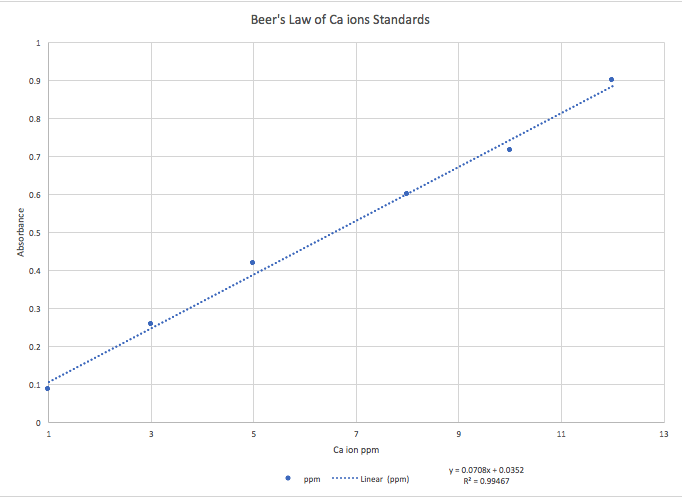
\includegraphics[width=5in]{fig1}\hspace*{\fill}
\caption[Beer's Law Calibration Plot for \ce{Ca} by Atomic Absorption (422.7 nm)]{Beer's Law Calibration Plot for \ce{Ca} by Atomic Absorption (422.7 nm)}
\end{figure}
\begin{enumerate}
    \item Example calculation for the preparation of one of the \ce{Ca} standards from the stock \ce{Ca} solution
    \begin{enumerate}
        \item $100 ppm \times 1\% = 1 ppm$
    \end{enumerate}
    \item The ppm (mg/L) of \ce{Ca} for each soil sample
    \begin{enumerate}
        \item $y = 0.0708x + 0.0352 \longrightarrow$ where $y = 0.491 (1:10)$\\$\longrightarrow 0.491 = 0.0708x + 0.0352 \longrightarrow x = \frac{0.491 - 0.0352}{0.0708} = 6.437$ \\ $\longrightarrow 6.44 \longrightarrow 6.44 \times$ $ 10 = 64.4 ppm$ for Soil 1 (1:10) \\ $\&$ Soil 3 (1:100) is $6.44 \times $ $100 = 644.0 ppm$
    \end{enumerate}
    \item Gravimetric analysis of soil additive
    \begin{enumerate}
        \item Initial mass of supplement used in the analysis by to heating
        \begin{enumerate}
            \item $33.31g -31.06g = 2.25g$
        \end{enumerate}
        \item Mass (g) of residue left after heating supplement
        \begin{enumerate}
            \item $32.64g - 31.06g = 1.58g$
        \end{enumerate}
        \item Mass (g) of \ce{CO_2} produced (mass lost after heating)
        \begin{enumerate}
            \item $33.31g - 32.64g = 0.67g$
        \end{enumerate}
        \item Mole of \ce{CO_2} produced after heating
        \begin{enumerate}
            \item $0.67g \times$ $ \frac{1 mol \ce{CO_2}}{44.01g} = 0.0152 mol \ce{CO_2}$
        \end{enumerate}
        \item Moles of \ce{CaCO_3} in the soil supplement
        \begin{enumerate}
            \item $0.0152 mol \ce{CO_2} \times$ $ \frac{1 mol \ce{CaCO_3}}{1 mol \ce{CO_2}} = 0.0152 mol \ce{CaCO_3}$
        \end{enumerate}
        \item Mass (g) of \ce{CaCO_3} in the soil supplement
        \begin{enumerate}
            \item $0.0152 mol \ce{CaCO_3} \times$ $ \frac{100g}{1 mol \ce{CaCO_3}} = 1.52g \ce{CaCO_3}$
        \end{enumerate}
        \item Weight percent ($\frac{w}{w}$)$\%$ of \ce{CaCO_3} in the soil supplement
        \begin{enumerate}
            \item $\frac{1.52g \ce{CaCO_3}}{2.25g} \times$ $ 100 = 67.6\%$
        \end{enumerate}
        \item Mass (g) of \ce{Na_2CO_3} in the soil supplement
         \begin{enumerate}
            \item $2.25g - 1.52g = 0.730g \ce{Na_2CO_3}$
        \end{enumerate}
        \item Weight percent ($\frac{w}{w}$)$\%$ of the \ce{Na_2CO_3} in the soil supplement
        \begin{enumerate}
            \item $\frac{0.730g \ce{Na_2CO_3}}{2.25g} \times$ $ 100 = 32.4\%$
        \end{enumerate}
        \item \ce{CaCO_3} ppm (mg/kg) in the soil supplement
        \begin{enumerate}
            \item  $\frac{1520mg \ce{CaCO_3}}{0.00225kg} = 644444.4 ppm$
        \end{enumerate}
    \end{enumerate}
\end{enumerate}
%----------------------------------------------------------------------------------------
%	SECTION 4
%----------------------------------------------------------------------------------------
\section{Results of calculations to be given in a table format}
\begin{table}[H]
\label{Table 9}
\caption{Results from the EDTA titration of soil eluents for their \ce{Ca}content}
\resizebox{45em}{!}{
\begin{tabular}{|l|l|l|l|l|}
\hline
\multicolumn{1}{|c|}{{\ul{\textbf{Soil #}}}} &
\multicolumn{1}{|C{5.0cm}|}{{\ul{\textbf{Average moles of \ce{Ca} in soil eluents}}}} &
\multicolumn{1}{|C{5.0cm}|}{{\ul{\textbf{Average grams of \ce{Ca} in soil sample per gram of soil ($\frac{w}{w}$)$\%$}}}} &
\multicolumn{1}{|C{5.0cm}|}{{\ul{\textbf{Average ppm (mg \ce{Ca} / kg of soil) of \ce{Ca} in soil sample}}}} &
\multicolumn{1}{|C{5.0cm}|}{{\ul{\textbf{Average molarity of \ce{Ca} in a soil sample}}}}\\ \hline
	 1 & $1.94\e{-5} mol \ce{Ca^2+}$ & 0.0154\% & 153.8ppm & 1.93\e{-4}M \\ \hline
	 3 & $1.50\e{-4} mol \ce{Ca^2+}$ & 0.1192\% & 1192.1ppm & 1.50\e{-3}M \\ \hline
	\end{tabular}
	}
	\centering
\end{table}

\begin{table}[H]
\label{Table 10}
\caption{Results from AA analysis of soil eluents for their \ce{Ca} content}
\resizebox{30em}{!}{
\begin{tabular}{|l|l|}
\hline
\multicolumn{1}{|c|}{{\ul{\textbf{Soil #}}}} &
\multicolumn{1}{c|}{{\ul{\textbf{ppm (mg/L) of \ce{Ca} for each soil sample}}}} \\ \hline
	 1 & 64.4 \\ \hline
	 3 & 644.0 \\ \hline
	\end{tabular}
	}
	\centering
\end{table}

\begin{table}[H]
\label{Table 11}
\caption{Results of Gravimetric analysis of \ce{CaCO_3 - Na_2CO_3} soil additive (mixture)}
\resizebox{45em}{!}{
\begin{tabular}{|l|l|l|l|}
\hline
\multicolumn{1}{|C{5.0cm}|}{{\ul{\textbf{Mass (g) of \ce{CaCO_3} in the additive (mixture)}}}} &
\multicolumn{1}{|C{5.0cm}|}{{\ul{\textbf{Weight percent ($\frac{w}{w}$)$\%$ of \ce{CaCO_3} in the additive}}}} &
\multicolumn{1}{|C{5.0cm}|}{{\ul{\textbf{Mass (g) of \ce{Na_2CO_3} in additive (mixture)}}}} &
\multicolumn{1}{|C{5.0cm}|}{{\ul{\textbf{Weight percent ($\frac{w}{w}$)$\%$ of \ce{Na_2CO_3} in the soil additive}}}}\\ \hline
	 1.52g & 67.6\% & 0.730g & 32.4\% \\ \hline

	\end{tabular}
	}
	\centering
\end{table}
%----------------------------------------------------------------------------------------
%	SECTION 5
%----------------------------------------------------------------------------------------
\section{Questions}
\hspace{5ex} The blank we used in this experiment was distilled water because we used in it preparation of the titration. There is \ce{Ca} in our water and we are checking for the amount of \ce{Ca} in soil we wouldn't want to exclude it from are calculations because then we could be inaccurate in our findings. For the atomic absorption (AA) spectroscopy analysis, he had six samples of \ce{Ca} that was diluted with varying amount of ppm standards (Table 5). We then used the information we got from the AA readings to a create Beer's plot (Figure 1) that graphically shows the \ce{Ca} levels in each of six samples. Also, we used distilled water as our blank because each of samples contained water. We want to know the absorbance value of water. So, we can take it out of our calculations. The AA creates a more accurate reading than relying on people say when it actually changes to the blue color. Considering many people have there own idea what blue is from there eyesight. If your colorblind and can't see certain colors then you would use a AA machine for more accuracy. Using a burette would create some precision but a difference between one more extra drop would change the accuracy of the data versus the AA. So in most cases, in case proven otherwise it's best to use a machine to avoid some deep error such as what one person may see as blue and the other violet. A common household product to increase \ce{Ca} in plants would be TUMS crushed down into powder form. Then spread across the soil for best absorption. When it rains or the soil gets wet the roots of the plant will get the nutrients. The ground may help in the filtering process as it gets to the roots.
%----------------------------------------------------------------------------------------
%	SECTION 6
%----------------------------------------------------------------------------------------
\bibliographystyle{IEEEtran}
\begin{thebibliography}{1}
\bibitem{Chem}
Department of Chemistry and Physics (2012). \textit{The Importance of Mineral Uptake in Plant Growth: Determination of Calcium Ion in Soil}. Armstrong State University, Savannah.
\end{thebibliography}
\end{document}
